% Created by tikzDevice version 0.10.1 on 2017-10-23 14:01:14
% !TEX encoding = UTF-8 Unicode
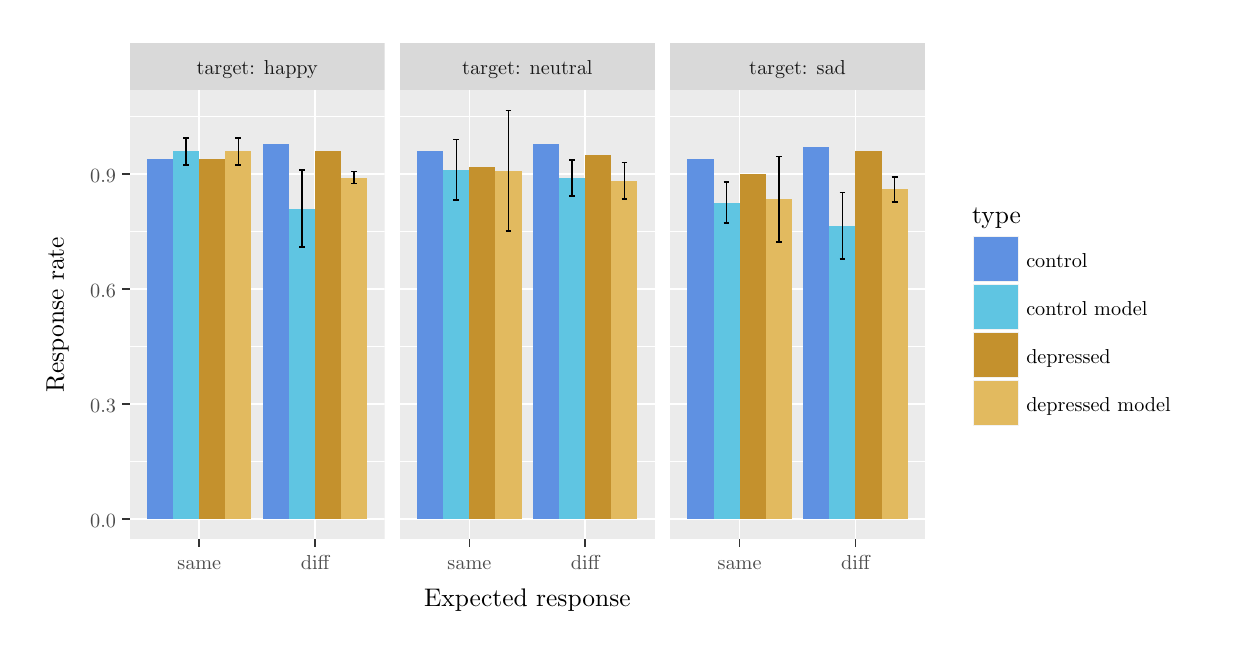
\begin{tikzpicture}[x=1pt,y=1pt]
\definecolor{fillColor}{RGB}{255,255,255}
\path[use as bounding box,fill=fillColor,fill opacity=0.00] (0,0) rectangle (433.62,216.81);
\begin{scope}
\path[clip] (  0.00,  0.00) rectangle (433.62,216.81);
\definecolor{drawColor}{RGB}{255,255,255}
\definecolor{fillColor}{RGB}{255,255,255}

\path[draw=drawColor,line width= 0.6pt,line join=round,line cap=round,fill=fillColor] ( -0.00,  0.00) rectangle (433.62,216.81);
\end{scope}
\begin{scope}
\path[clip] ( 36.87, 31.92) rectangle (129.00,194.25);
\definecolor{fillColor}{gray}{0.92}

\path[fill=fillColor] ( 36.87, 31.92) rectangle (129.00,194.25);
\definecolor{drawColor}{RGB}{255,255,255}

\path[draw=drawColor,line width= 0.3pt,line join=round] ( 36.87, 60.05) --
	(129.00, 60.05);

\path[draw=drawColor,line width= 0.3pt,line join=round] ( 36.87,101.56) --
	(129.00,101.56);

\path[draw=drawColor,line width= 0.3pt,line join=round] ( 36.87,143.07) --
	(129.00,143.07);

\path[draw=drawColor,line width= 0.3pt,line join=round] ( 36.87,184.58) --
	(129.00,184.58);

\path[draw=drawColor,line width= 0.6pt,line join=round] ( 36.87, 39.30) --
	(129.00, 39.30);

\path[draw=drawColor,line width= 0.6pt,line join=round] ( 36.87, 80.81) --
	(129.00, 80.81);

\path[draw=drawColor,line width= 0.6pt,line join=round] ( 36.87,122.32) --
	(129.00,122.32);

\path[draw=drawColor,line width= 0.6pt,line join=round] ( 36.87,163.83) --
	(129.00,163.83);

\path[draw=drawColor,line width= 0.6pt,line join=round] ( 61.99, 31.92) --
	( 61.99,194.25);

\path[draw=drawColor,line width= 0.6pt,line join=round] (103.87, 31.92) --
	(103.87,194.25);
\definecolor{fillColor}{RGB}{226,186,95}

\path[fill=fillColor] ( 71.41, 39.30) rectangle ( 80.84,172.16);
\definecolor{fillColor}{RGB}{196,145,45}

\path[fill=fillColor] ( 61.99, 39.30) rectangle ( 71.41,169.36);
\definecolor{fillColor}{RGB}{95,197,226}

\path[fill=fillColor] ( 52.57, 39.30) rectangle ( 61.99,172.07);
\definecolor{fillColor}{RGB}{95,145,226}

\path[fill=fillColor] ( 43.15, 39.30) rectangle ( 52.57,169.36);
\definecolor{fillColor}{RGB}{226,186,95}

\path[fill=fillColor] (113.29, 39.30) rectangle (122.71,162.63);
\definecolor{fillColor}{RGB}{196,145,45}

\path[fill=fillColor] (103.87, 39.30) rectangle (113.29,172.13);
\definecolor{fillColor}{RGB}{95,197,226}

\path[fill=fillColor] ( 94.45, 39.30) rectangle (103.87,151.45);
\definecolor{fillColor}{RGB}{95,145,226}

\path[fill=fillColor] ( 85.02, 39.30) rectangle ( 94.45,174.90);
\definecolor{drawColor}{RGB}{0,0,0}

\path[draw=drawColor,line width= 0.6pt,line join=round] ( 75.08,177.02) --
	( 77.17,177.02);

\path[draw=drawColor,line width= 0.6pt,line join=round] ( 76.13,177.02) --
	( 76.13,167.30);

\path[draw=drawColor,line width= 0.6pt,line join=round] ( 75.08,167.30) --
	( 77.17,167.30);

\path[draw=drawColor,line width= 0.6pt,line join=round] ( 56.23,176.92) --
	( 58.33,176.92);

\path[draw=drawColor,line width= 0.6pt,line join=round] ( 57.28,176.92) --
	( 57.28,167.21);

\path[draw=drawColor,line width= 0.6pt,line join=round] ( 56.23,167.21) --
	( 58.33,167.21);

\path[draw=drawColor,line width= 0.6pt,line join=round] (116.96,164.80) --
	(119.05,164.80);

\path[draw=drawColor,line width= 0.6pt,line join=round] (118.00,164.80) --
	(118.00,160.46);

\path[draw=drawColor,line width= 0.6pt,line join=round] (116.96,160.46) --
	(119.05,160.46);

\path[draw=drawColor,line width= 0.6pt,line join=round] ( 98.11,165.32) --
	(100.20,165.32);

\path[draw=drawColor,line width= 0.6pt,line join=round] ( 99.16,165.32) --
	( 99.16,137.58);

\path[draw=drawColor,line width= 0.6pt,line join=round] ( 98.11,137.58) --
	(100.20,137.58);
\end{scope}
\begin{scope}
\path[clip] (134.50, 31.92) rectangle (226.62,194.25);
\definecolor{fillColor}{gray}{0.92}

\path[fill=fillColor] (134.50, 31.92) rectangle (226.62,194.25);
\definecolor{drawColor}{RGB}{255,255,255}

\path[draw=drawColor,line width= 0.3pt,line join=round] (134.50, 60.05) --
	(226.62, 60.05);

\path[draw=drawColor,line width= 0.3pt,line join=round] (134.50,101.56) --
	(226.62,101.56);

\path[draw=drawColor,line width= 0.3pt,line join=round] (134.50,143.07) --
	(226.62,143.07);

\path[draw=drawColor,line width= 0.3pt,line join=round] (134.50,184.58) --
	(226.62,184.58);

\path[draw=drawColor,line width= 0.6pt,line join=round] (134.50, 39.30) --
	(226.62, 39.30);

\path[draw=drawColor,line width= 0.6pt,line join=round] (134.50, 80.81) --
	(226.62, 80.81);

\path[draw=drawColor,line width= 0.6pt,line join=round] (134.50,122.32) --
	(226.62,122.32);

\path[draw=drawColor,line width= 0.6pt,line join=round] (134.50,163.83) --
	(226.62,163.83);

\path[draw=drawColor,line width= 0.6pt,line join=round] (159.62, 31.92) --
	(159.62,194.25);

\path[draw=drawColor,line width= 0.6pt,line join=round] (201.50, 31.92) --
	(201.50,194.25);
\definecolor{fillColor}{RGB}{226,186,95}

\path[fill=fillColor] (169.04, 39.30) rectangle (178.47,165.08);
\definecolor{fillColor}{RGB}{196,145,45}

\path[fill=fillColor] (159.62, 39.30) rectangle (169.04,166.59);
\definecolor{fillColor}{RGB}{95,197,226}

\path[fill=fillColor] (150.20, 39.30) rectangle (159.62,165.44);
\definecolor{fillColor}{RGB}{95,145,226}

\path[fill=fillColor] (140.78, 39.30) rectangle (150.20,172.13);
\definecolor{fillColor}{RGB}{226,186,95}

\path[fill=fillColor] (210.92, 39.30) rectangle (220.34,161.53);
\definecolor{fillColor}{RGB}{196,145,45}

\path[fill=fillColor] (201.50, 39.30) rectangle (210.92,170.74);
\definecolor{fillColor}{RGB}{95,197,226}

\path[fill=fillColor] (192.08, 39.30) rectangle (201.50,162.44);
\definecolor{fillColor}{RGB}{95,145,226}

\path[fill=fillColor] (182.65, 39.30) rectangle (192.08,174.90);
\definecolor{drawColor}{RGB}{0,0,0}

\path[draw=drawColor,line width= 0.6pt,line join=round] (172.71,186.87) --
	(174.80,186.87);

\path[draw=drawColor,line width= 0.6pt,line join=round] (173.75,186.87) --
	(173.75,143.30);

\path[draw=drawColor,line width= 0.6pt,line join=round] (172.71,143.30) --
	(174.80,143.30);

\path[draw=drawColor,line width= 0.6pt,line join=round] (153.86,176.43) --
	(155.96,176.43);

\path[draw=drawColor,line width= 0.6pt,line join=round] (154.91,176.43) --
	(154.91,154.45);

\path[draw=drawColor,line width= 0.6pt,line join=round] (153.86,154.45) --
	(155.96,154.45);

\path[draw=drawColor,line width= 0.6pt,line join=round] (214.58,168.05) --
	(216.68,168.05);

\path[draw=drawColor,line width= 0.6pt,line join=round] (215.63,168.05) --
	(215.63,155.01);

\path[draw=drawColor,line width= 0.6pt,line join=round] (214.58,155.01) --
	(216.68,155.01);

\path[draw=drawColor,line width= 0.6pt,line join=round] (195.74,168.94) --
	(197.83,168.94);

\path[draw=drawColor,line width= 0.6pt,line join=round] (196.79,168.94) --
	(196.79,155.93);

\path[draw=drawColor,line width= 0.6pt,line join=round] (195.74,155.93) --
	(197.83,155.93);
\end{scope}
\begin{scope}
\path[clip] (232.12, 31.92) rectangle (324.25,194.25);
\definecolor{fillColor}{gray}{0.92}

\path[fill=fillColor] (232.12, 31.92) rectangle (324.25,194.25);
\definecolor{drawColor}{RGB}{255,255,255}

\path[draw=drawColor,line width= 0.3pt,line join=round] (232.12, 60.05) --
	(324.25, 60.05);

\path[draw=drawColor,line width= 0.3pt,line join=round] (232.12,101.56) --
	(324.25,101.56);

\path[draw=drawColor,line width= 0.3pt,line join=round] (232.12,143.07) --
	(324.25,143.07);

\path[draw=drawColor,line width= 0.3pt,line join=round] (232.12,184.58) --
	(324.25,184.58);

\path[draw=drawColor,line width= 0.6pt,line join=round] (232.12, 39.30) --
	(324.25, 39.30);

\path[draw=drawColor,line width= 0.6pt,line join=round] (232.12, 80.81) --
	(324.25, 80.81);

\path[draw=drawColor,line width= 0.6pt,line join=round] (232.12,122.32) --
	(324.25,122.32);

\path[draw=drawColor,line width= 0.6pt,line join=round] (232.12,163.83) --
	(324.25,163.83);

\path[draw=drawColor,line width= 0.6pt,line join=round] (257.25, 31.92) --
	(257.25,194.25);

\path[draw=drawColor,line width= 0.6pt,line join=round] (299.13, 31.92) --
	(299.13,194.25);
\definecolor{fillColor}{RGB}{226,186,95}

\path[fill=fillColor] (266.67, 39.30) rectangle (276.09,154.82);
\definecolor{fillColor}{RGB}{196,145,45}

\path[fill=fillColor] (257.25, 39.30) rectangle (266.67,163.83);
\definecolor{fillColor}{RGB}{95,197,226}

\path[fill=fillColor] (247.83, 39.30) rectangle (257.25,153.57);
\definecolor{fillColor}{RGB}{95,145,226}

\path[fill=fillColor] (238.41, 39.30) rectangle (247.83,169.36);
\definecolor{fillColor}{RGB}{226,186,95}

\path[fill=fillColor] (308.55, 39.30) rectangle (317.97,158.41);
\definecolor{fillColor}{RGB}{196,145,45}

\path[fill=fillColor] (299.13, 39.30) rectangle (308.55,172.13);
\definecolor{fillColor}{RGB}{95,197,226}

\path[fill=fillColor] (289.70, 39.30) rectangle (299.13,145.19);
\definecolor{fillColor}{RGB}{95,145,226}

\path[fill=fillColor] (280.28, 39.30) rectangle (289.70,173.51);
\definecolor{drawColor}{RGB}{0,0,0}

\path[draw=drawColor,line width= 0.6pt,line join=round] (270.34,170.21) --
	(272.43,170.21);

\path[draw=drawColor,line width= 0.6pt,line join=round] (271.38,170.21) --
	(271.38,139.44);

\path[draw=drawColor,line width= 0.6pt,line join=round] (270.34,139.44) --
	(272.43,139.44);

\path[draw=drawColor,line width= 0.6pt,line join=round] (251.49,160.94) --
	(253.59,160.94);

\path[draw=drawColor,line width= 0.6pt,line join=round] (252.54,160.94) --
	(252.54,146.20);

\path[draw=drawColor,line width= 0.6pt,line join=round] (251.49,146.20) --
	(253.59,146.20);

\path[draw=drawColor,line width= 0.6pt,line join=round] (312.21,162.93) --
	(314.31,162.93);

\path[draw=drawColor,line width= 0.6pt,line join=round] (313.26,162.93) --
	(313.26,153.89);

\path[draw=drawColor,line width= 0.6pt,line join=round] (312.21,153.89) --
	(314.31,153.89);

\path[draw=drawColor,line width= 0.6pt,line join=round] (293.37,157.26) --
	(295.46,157.26);

\path[draw=drawColor,line width= 0.6pt,line join=round] (294.42,157.26) --
	(294.42,133.12);

\path[draw=drawColor,line width= 0.6pt,line join=round] (293.37,133.12) --
	(295.46,133.12);
\end{scope}
\begin{scope}
\path[clip] ( 36.87,194.25) rectangle (129.00,211.31);
\definecolor{fillColor}{gray}{0.85}

\path[fill=fillColor] ( 36.87,194.25) rectangle (129.00,211.31);
\definecolor{drawColor}{gray}{0.10}

\node[text=drawColor,anchor=base,inner sep=0pt, outer sep=0pt, scale=  0.73] at ( 82.93,199.75) {target: happy};
\end{scope}
\begin{scope}
\path[clip] (134.50,194.25) rectangle (226.62,211.31);
\definecolor{fillColor}{gray}{0.85}

\path[fill=fillColor] (134.50,194.25) rectangle (226.62,211.31);
\definecolor{drawColor}{gray}{0.10}

\node[text=drawColor,anchor=base,inner sep=0pt, outer sep=0pt, scale=  0.73] at (180.56,199.75) {target: neutral};
\end{scope}
\begin{scope}
\path[clip] (232.12,194.25) rectangle (324.25,211.31);
\definecolor{fillColor}{gray}{0.85}

\path[fill=fillColor] (232.12,194.25) rectangle (324.25,211.31);
\definecolor{drawColor}{gray}{0.10}

\node[text=drawColor,anchor=base,inner sep=0pt, outer sep=0pt, scale=  0.73] at (278.19,199.75) {target: sad};
\end{scope}
\begin{scope}
\path[clip] (  0.00,  0.00) rectangle (433.62,216.81);
\definecolor{drawColor}{gray}{0.20}

\path[draw=drawColor,line width= 0.6pt,line join=round] ( 61.99, 29.17) --
	( 61.99, 31.92);

\path[draw=drawColor,line width= 0.6pt,line join=round] (103.87, 29.17) --
	(103.87, 31.92);
\end{scope}
\begin{scope}
\path[clip] (  0.00,  0.00) rectangle (433.62,216.81);
\definecolor{drawColor}{gray}{0.30}

\node[text=drawColor,anchor=base,inner sep=0pt, outer sep=0pt, scale=  0.73] at ( 61.99, 20.91) {same};

\node[text=drawColor,anchor=base,inner sep=0pt, outer sep=0pt, scale=  0.73] at (103.87, 20.91) {diff};
\end{scope}
\begin{scope}
\path[clip] (  0.00,  0.00) rectangle (433.62,216.81);
\definecolor{drawColor}{gray}{0.20}

\path[draw=drawColor,line width= 0.6pt,line join=round] (159.62, 29.17) --
	(159.62, 31.92);

\path[draw=drawColor,line width= 0.6pt,line join=round] (201.50, 29.17) --
	(201.50, 31.92);
\end{scope}
\begin{scope}
\path[clip] (  0.00,  0.00) rectangle (433.62,216.81);
\definecolor{drawColor}{gray}{0.30}

\node[text=drawColor,anchor=base,inner sep=0pt, outer sep=0pt, scale=  0.73] at (159.62, 20.91) {same};

\node[text=drawColor,anchor=base,inner sep=0pt, outer sep=0pt, scale=  0.73] at (201.50, 20.91) {diff};
\end{scope}
\begin{scope}
\path[clip] (  0.00,  0.00) rectangle (433.62,216.81);
\definecolor{drawColor}{gray}{0.20}

\path[draw=drawColor,line width= 0.6pt,line join=round] (257.25, 29.17) --
	(257.25, 31.92);

\path[draw=drawColor,line width= 0.6pt,line join=round] (299.13, 29.17) --
	(299.13, 31.92);
\end{scope}
\begin{scope}
\path[clip] (  0.00,  0.00) rectangle (433.62,216.81);
\definecolor{drawColor}{gray}{0.30}

\node[text=drawColor,anchor=base,inner sep=0pt, outer sep=0pt, scale=  0.73] at (257.25, 20.91) {same};

\node[text=drawColor,anchor=base,inner sep=0pt, outer sep=0pt, scale=  0.73] at (299.13, 20.91) {diff};
\end{scope}
\begin{scope}
\path[clip] (  0.00,  0.00) rectangle (433.62,216.81);
\definecolor{drawColor}{gray}{0.30}

\node[text=drawColor,anchor=base east,inner sep=0pt, outer sep=0pt, scale=  0.73] at ( 31.92, 36.27) {0.0};

\node[text=drawColor,anchor=base east,inner sep=0pt, outer sep=0pt, scale=  0.73] at ( 31.92, 77.78) {0.3};

\node[text=drawColor,anchor=base east,inner sep=0pt, outer sep=0pt, scale=  0.73] at ( 31.92,119.29) {0.6};

\node[text=drawColor,anchor=base east,inner sep=0pt, outer sep=0pt, scale=  0.73] at ( 31.92,160.80) {0.9};
\end{scope}
\begin{scope}
\path[clip] (  0.00,  0.00) rectangle (433.62,216.81);
\definecolor{drawColor}{gray}{0.20}

\path[draw=drawColor,line width= 0.6pt,line join=round] ( 34.12, 39.30) --
	( 36.87, 39.30);

\path[draw=drawColor,line width= 0.6pt,line join=round] ( 34.12, 80.81) --
	( 36.87, 80.81);

\path[draw=drawColor,line width= 0.6pt,line join=round] ( 34.12,122.32) --
	( 36.87,122.32);

\path[draw=drawColor,line width= 0.6pt,line join=round] ( 34.12,163.83) --
	( 36.87,163.83);
\end{scope}
\begin{scope}
\path[clip] (  0.00,  0.00) rectangle (433.62,216.81);
\definecolor{drawColor}{RGB}{0,0,0}

\node[text=drawColor,anchor=base,inner sep=0pt, outer sep=0pt, scale=  0.92] at (180.56,  7.83) {Expected response};
\end{scope}
\begin{scope}
\path[clip] (  0.00,  0.00) rectangle (433.62,216.81);
\definecolor{drawColor}{RGB}{0,0,0}

\node[text=drawColor,rotate= 90.00,anchor=base,inner sep=0pt, outer sep=0pt, scale=  0.92] at ( 13.08,113.08) {Response rate};
\end{scope}
\begin{scope}
\path[clip] (  0.00,  0.00) rectangle (433.62,216.81);
\definecolor{fillColor}{RGB}{255,255,255}

\path[fill=fillColor] (335.63, 66.75) rectangle (428.12,159.42);
\end{scope}
\begin{scope}
\path[clip] (  0.00,  0.00) rectangle (433.62,216.81);
\definecolor{drawColor}{RGB}{0,0,0}

\node[text=drawColor,anchor=base west,inner sep=0pt, outer sep=0pt, scale=  0.92] at (341.32,146.15) {type};
\end{scope}
\begin{scope}
\path[clip] (  0.00,  0.00) rectangle (433.62,216.81);
\definecolor{drawColor}{RGB}{255,255,255}
\definecolor{fillColor}{gray}{0.95}

\path[draw=drawColor,line width= 0.6pt,line join=round,line cap=round,fill=fillColor] (341.32,124.47) rectangle (358.67,141.82);
\end{scope}
\begin{scope}
\path[clip] (  0.00,  0.00) rectangle (433.62,216.81);
\definecolor{fillColor}{RGB}{95,145,226}

\path[fill=fillColor] (342.04,125.18) rectangle (357.96,141.11);
\end{scope}
\begin{scope}
\path[clip] (  0.00,  0.00) rectangle (433.62,216.81);
\definecolor{drawColor}{RGB}{255,255,255}
\definecolor{fillColor}{gray}{0.95}

\path[draw=drawColor,line width= 0.6pt,line join=round,line cap=round,fill=fillColor] (341.32,107.13) rectangle (358.67,124.47);
\end{scope}
\begin{scope}
\path[clip] (  0.00,  0.00) rectangle (433.62,216.81);
\definecolor{fillColor}{RGB}{95,197,226}

\path[fill=fillColor] (342.04,107.84) rectangle (357.96,123.76);
\end{scope}
\begin{scope}
\path[clip] (  0.00,  0.00) rectangle (433.62,216.81);
\definecolor{drawColor}{RGB}{255,255,255}
\definecolor{fillColor}{gray}{0.95}

\path[draw=drawColor,line width= 0.6pt,line join=round,line cap=round,fill=fillColor] (341.32, 89.78) rectangle (358.67,107.13);
\end{scope}
\begin{scope}
\path[clip] (  0.00,  0.00) rectangle (433.62,216.81);
\definecolor{fillColor}{RGB}{196,145,45}

\path[fill=fillColor] (342.04, 90.49) rectangle (357.96,106.42);
\end{scope}
\begin{scope}
\path[clip] (  0.00,  0.00) rectangle (433.62,216.81);
\definecolor{drawColor}{RGB}{255,255,255}
\definecolor{fillColor}{gray}{0.95}

\path[draw=drawColor,line width= 0.6pt,line join=round,line cap=round,fill=fillColor] (341.32, 72.44) rectangle (358.67, 89.78);
\end{scope}
\begin{scope}
\path[clip] (  0.00,  0.00) rectangle (433.62,216.81);
\definecolor{fillColor}{RGB}{226,186,95}

\path[fill=fillColor] (342.04, 73.15) rectangle (357.96, 89.07);
\end{scope}
\begin{scope}
\path[clip] (  0.00,  0.00) rectangle (433.62,216.81);
\definecolor{drawColor}{RGB}{0,0,0}

\node[text=drawColor,anchor=base west,inner sep=0pt, outer sep=0pt, scale=  0.73] at (360.84,130.12) {control};
\end{scope}
\begin{scope}
\path[clip] (  0.00,  0.00) rectangle (433.62,216.81);
\definecolor{drawColor}{RGB}{0,0,0}

\node[text=drawColor,anchor=base west,inner sep=0pt, outer sep=0pt, scale=  0.73] at (360.84,112.77) {control model};
\end{scope}
\begin{scope}
\path[clip] (  0.00,  0.00) rectangle (433.62,216.81);
\definecolor{drawColor}{RGB}{0,0,0}

\node[text=drawColor,anchor=base west,inner sep=0pt, outer sep=0pt, scale=  0.73] at (360.84, 95.43) {depressed};
\end{scope}
\begin{scope}
\path[clip] (  0.00,  0.00) rectangle (433.62,216.81);
\definecolor{drawColor}{RGB}{0,0,0}

\node[text=drawColor,anchor=base west,inner sep=0pt, outer sep=0pt, scale=  0.73] at (360.84, 78.08) {depressed model};
\end{scope}
\end{tikzpicture}
